\documentclass[10pt]{IEEEtran}
\usepackage[spanish]{babel}
\usepackage[utf8]{inputenc}
\usepackage{graphicx}
\usepackage{subfigure} 
\usepackage{amsmath}
\usepackage{float}



\title {Cifrado parcial. Reporte 1.}

\author{\IEEEauthorblockN{Marcos Daniel Calderón Calderón}\\
\IEEEauthorblockA{Maestría en Ciencias de la Computación\\
Centro de Investigación en Matemáticas (CIMAT)\\
Guanajuato , Gto.\\
marcos.calderon@cimat.mx}}


\begin{document}
\maketitle
\begin{abstract}
En este documento se explica detallada el proceso de implementación de un programa de cifrado parcial.
\end{abstract}
\section{Descripción del proceso.}

\subsection{Inversión de bits.}
En el proceso de inversión de bits, se toman en cuenta los siguientes parámetros:
\begin{itemize}
\item \textbf{Av}. Esta cantidad es el promedio promido de los códigos de Huffman que se obtienen después de aplicar un algoritmo de compresión a los datos transmitidos. Esta cantidad se calcula por medio de la siguiente espresión:


\begin{equation}
Av = \sum_{i=1}^{N}P(C_{i})L(C_{i})
\end{equation}

donde $P(C_{i})$ es la probabilidad de obtener el simbolo que representa el código. y $L(C_{i})$ es la longitud del código indicado.
 
\item \textbf{db}. Supongamos que estamos en un bloque de tamaño $Av$ bits, y tomamos como referencia un bit $B_{i}$ que es encuentra en la posición $i$, y que está en el interior del bloque, entones $db$ es la distancia en bits del bit $B_{i}$ al inicio del bloque.  

\item \textbf{de}. Supongamos que estamos en un bloque de tamaño $Av$ bits, y tomamos como referencia un bit $B_{i}$ que es encuentra en la posición $i$, y que está en el interior del bloque, $de$ es la distancia en bits del bit $B_{i}$ al final del bloque.  
  
\end{itemize}


Con base en las especificaciones anteriores, existen dos maneras de lograr la inversión de bits:


\begin{enumerate}
\item Elige una posición aleatoria: $Pos= randomChaoticNumber \mod{Av}$ de los primeros $Av$ bits del paquete y calcula la distancia de este punto al inicio y fin del bloque (\textbf{db} y \textbf{de} respecivamente).


\item Si el número aleatorio es par, se elige la siguiente posición de bit a invertir: $flipbitPos = randomNumber \mod{db} $. Si el número aleatorio es impar entonces: $flipbitPos = randomNumber \mod{de}$. Lo anterior significa que de la posición de referencia, ''arrojamos una moneda'' para decidir la dirección del bit a invertir.


\item Ahora, el proceso de inversión de bits por todo el paquete puede hacerse de varias formas, a continuación mencionamos las principales que además, se pueden combinar.

\begin{itemize}
\item Ir al siguiente bloque y repetir los pasos 1 y 2. El inicio del siguiente bloque es el nuevo puntgo global de referencia para el siguiente cálculo de inversión de bit. La debilidad de este método es que pueden ocurrir huecos extensos (más grandes que $Av$) entre dos bits invertidos. 


\item La posición del último bit ivertido es el nuevo punto de referencia para el siguiente bit a invertir. Y se repiten los pasos 1 y 2. Para considerar difusión, el punto de referencia en la actual iteracion se calcula de la siguiente manera:


\begin{equation}
Pos = PrevChaoticN+
NewChaoticN \mod{Av}
\end{equation}


\end{itemize}



\end{enumerate}



\subsection{Permutación de segmentos.}

El proceso de permutación de segmentos ocurre de la siguiente manera:


\begin{enumerate}
\item Cada uno de los paquetes RTP  lo dividimos en segmentos. Éstos ejemplos son lo que se permutarán. Se aplicó el siguiente esquema de permutación que indica la figura  ~\ref{kaa}.

\begin{figure}[H]
\centering
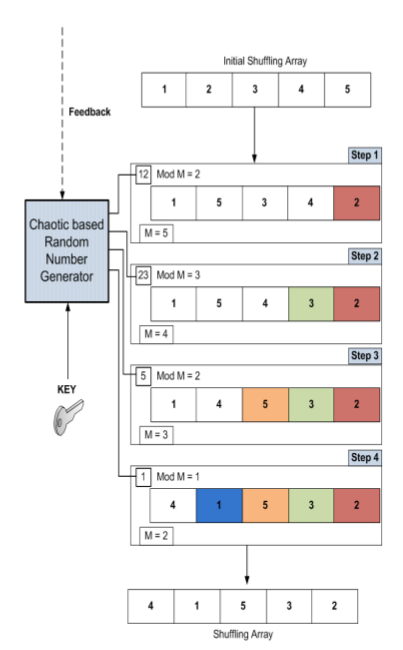
\includegraphics[width=7cm]{per.png}
\caption{Esquema 1.}
\label{kaa}
\end{figure}

\end{enumerate}

\subsubsection{Algunos resultados obtenidos.}
Para poder visualizar los resultados, supongamos que tenemos los datos de la imagen \textbf{lena}, y hacemos permutación de segmentos. Obtenemos los siguientes resultados ~\ref{ru}.


\begin{figure}[H]
\centering

\includegraphics[width=7cm]{lena.jpg}
\caption{Imagen Original.}
\label{ras}
\end{figure}

\begin{figure}[H]
\centering

\includegraphics[width=7cm]{final.jpg}
\caption{Resultado.}
\label{ru}
\end{figure}


Se tomaron en cuenta los siguientes aspectos para el ejemplo anterior:

\begin{enumerate}
\item El tamaño del paquete fué de 300 bytes.
\item EL tamaño del archivo fué de 13246 bytes.
\item Con base en los dos puntos anteriores, se pudieron encontrar 44 paquetes.

\end{enumerate}




\onecolumn

\section{Anexos.}



\subsection{Código para permutar segmentos.}
\begin{verbatim}
/*********** Proceso de cifrado para cada uno de los paquetes RTP ******************/

for(irtp=0; irtp < numPaquetesRTP; irtp++ ){

        /*=================== Proceso de Permutacion ==============================*/	
		srand (time(NULL));
		M=20;
		for(iSeg =1; iSeg < Lsegmentos; iSeg++){
			M=M-1;
			R= rand(); //Generate random number R
			T= R%M;
		
	    		/*Ahora, hacemos el intercambio que sea necesario.*/
       		for(iTamSeg=0; iTamSeg<tamanioSegmento; iTamSeg++){
				posicion1=(tamanioSegmento*(T)+iTamSeg) + (irtp*tamanioPaqueteRTP);
				posicion2=(tamanioSegmento*(M)+iTamSeg) + (irtp*tamanioPaqueteRTP);

				auxiliar = datosArchivo[posicion1];
				datosArchivo[posicion1]=datosArchivo[posicion2];
				datosArchivo[posicion2]= auxiliar;
	    		}	
	    }
        /*=========================================================================*/
}

/***********************************************************************************/
\end{verbatim}



\subsection{Código para inversión de bits, (sólo el primer segmento).}

\begin{verbatim}

        for(irtp=0; irtp < numPaquetesRTP; irtp++ ){
		/*El tamanio del archivo es de */
                
                /*Tabajamos con el primer octeto de codigo.*/
                refRTP=tamRTP*irtp;
                aleatorio=rand()+1;
                bitRef=(aleatorio %(avCodigo-2))+1;
                db=bitRef;//Bits a la izquierda
                de= avCodigo -(bitRef+1);
	

               /*Si el numero aleatorio es par...*/
                if((aleatorio%2)==0){  
					if(db!=0){
						posicionInversion=(aleatorio%db)+1;
						textos[0+irtp*tamRTP]= textos[0+irtp*tamRTP]
						^
						(1<<(avCodigo - (db-posicionInversion+1)));                  
					}
                }
	            /*Si el numero aleatorio es impar...*/
                else{
		            if(de!=0){		
				        posicionInversion=(aleatorio%de)+1;
			
		                textos[0+irtp*tamRTP]=
		                textos[0+irtp*tamRTP]
		                ^
		                (1<<(de - posicionInversion));                              
			        }
                }

        }


\end{verbatim}

\end{document}


